\begin{frame}{BitTorrent}
    \begin{itemize}
    \item tool for lots of people downloading big file
        \begin{itemize}
        \item example: install disk for Linux distribution
        \item (yes, there are some not-so-great examples)
        \end{itemize}
    \item goal: everyone helps each other download the file
        \begin{itemize}
        \item rather than making it the job of a few overloaded servers
        \item take advantage of `spare' bandwidth
        \end{itemize}
    \item can also use these ideas for transferring files within a network
    \end{itemize}
\end{frame}

\begin{frame}{`torrent' files}
    \begin{itemize}
    \item torrent files:
        \begin{itemize}
        \item a summary of the big file
        \item `tracker' information
        \end{itemize}
    \item list of the cryptographic hashes of every X bytes of the file
        \begin{itemize}
        \item typical X: 256KB-1MB
        \end{itemize}
    \vspace{.5cm}
    \item then: can verify if we have piece Y
    \item \ldots so don't care where it comes from
    \end{itemize}
\end{frame}

\begin{frame}{download from everyone (1)}
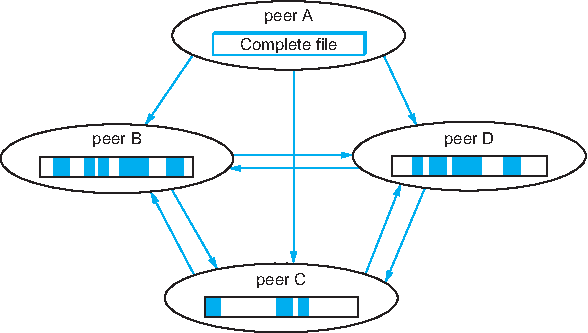
\includegraphics[height=0.9\textheight]{sysapp-bittorrent.pdf}
\end{frame}

\begin{frame}{download from everyone (2)}
    \begin{itemize}
    \item if A has whole file (parts 1--12), B has parts 1, 3, 5; C has parts 2, 4, 7.
    \vspace{.5cm}
    \item then possible plan:
        \begin{itemize}
        \item get parts 5, 6, 8, 9, 10, 11, 12 from A
        \item get parts 1, 3, 5 from B
        \item get parts 2, 4, 7 from C
        \end{itemize}
    \item but better than that:
        \begin{itemize}
        \item B and C are also downloading file, probably
        \item they'll have more parts later!
        \end{itemize}
    \end{itemize}
\end{frame}

\begin{frame}{a planning question}
    \begin{itemize}
    \item if A has whole file (parts 1--12), B has parts 1, 3, 5; C has parts 2, 4, 7.
    \vspace{.5cm}
    \item could spend a lot of effort planning who sends what to whom\ldotsS
    \item but\ldots
        \begin{itemize}
        \item no central authority
        \item nodes drop in/out of network
        \item lots of nodes in practice
        \end{itemize}
    \item so simpler typical solution: get random available piece
    \end{itemize}
\end{frame}

\begin{frame}{randomness allows sharing}
    \begin{itemize}
    \item suppose A and B are both downloading a file
    \item if they both did it in same order --- only sharing in one direction
        \begin{itemize}
        \item also true if they both prioritize in the same way
        \end{itemize}
    \item if they do it in random order
        \begin{itemize}
        \item if both have 20\% of file, probably only around 20\% overlap by chance
        \end{itemize}
    \end{itemize}
\end{frame}

\begin{frame}{freeriding}
    \begin{itemize}
    \item user goal: one wants to download file
    \item \ldots often little incentive to help others download
    \vspace{.5cm}
    \item could just reject requests to download\ldots
    \item or make them go superslow
    \end{itemize}
\end{frame}

\begin{frame}{tit-for-tat}
    \begin{itemize}
    \item algorithm to encourage uploading:
    \vspace{.5cm}
    \item when choosing who to upload to\ldots
    \item prefer requests for nodes that have uploaded to you
    \item `choke' nodes that have not in a while
        \begin{itemize}
        \item at least if you have `better' choices to upload to
        \end{itemize}
    \end{itemize}
\end{frame}

\begin{frame}{trackers}
    \begin{itemize}
    \item still need to find peers
    \vspace{.5cm}
    \item original BitTorrent solution: trackers run over HTTP
    \item peers periodically make HTTP request with their info
    \item tracker maintains database of recent peers
    \item returns a list of possible peers and their addresses
    \vspace{.5cm}
    \item later: decentralized solution
    \end{itemize}
\end{frame}
